\documentclass[article]{jss}

%% -- LaTeX packages and custom commands ---------------------------------------

%% recommended packages
\usepackage{thumbpdf,lmodern}

%% another package (only for this demo article)
\usepackage{framed}

%% new custom commands
\newcommand{\class}[1]{`\code{#1}'}
\newcommand{\fct}[1]{\code{#1()}}


%% -- Article metainformation (author, title, ...) -----------------------------

%% - \author{} with primary affiliation
%% - \Plainauthor{} without affiliations
%% - Separate authors by \And or \AND (in \author) or by comma (in \Plainauthor).
%% - \AND starts a new line, \And does not.
\author{Achim Zeileis\\Universit\"at Innsbruck
   \And Second Author\\Plus Affiliation}
\Plainauthor{Achim Zeileis, Second Author}

%% - \title{} in title case
%% - \Plaintitle{} without LaTeX markup (if any)
%% - \Shorttitle{} with LaTeX markup (if any), used as running title
\title{A Short Demo Article: Regression Models for Count Data in \proglang{R}}
\Plaintitle{A Short Demo Article: Regression Models for Count Data in R}
\Shorttitle{A Short Demo Article in \proglang{R}}

%% - \Abstract{} almost as usual
\Abstract{
  This short article illustrates how to write a manuscript for the
  \emph{Journal of Statistical Software} (JSS) using its {\LaTeX} style files.
  Generally, we ask to follow JSS's style guide and FAQs precisely. Also,
  it is recommended to keep the {\LaTeX} code as simple as possible,
  i.e., avoid inclusion of packages/commands that are not necessary.
  For outlining the typical structure of a JSS article some brief text snippets
  are employed that have been inspired by \cite{Zeileis+Kleiber+Jackman:2008},
  discussing count data regression in \proglang{R}. Editorial comments and
  instructions are marked by vertical bars.
}

%% - \Keywords{} with LaTeX markup, at least one required
%% - \Plainkeywords{} without LaTeX markup (if necessary)
%% - Should be comma-separated and in sentence case.
\Keywords{JSS, style guide, comma-separated, not capitalized, \proglang{R}}
\Plainkeywords{JSS, style guide, comma-separated, not capitalized, R}

%% - \Address{} of at least one author
%% - May contain multiple affiliations for each author
%%   (in extra lines, separated by \emph{and}\\).
%% - May contain multiple authors for the same affiliation
%%   (in the same first line, separated by comma).
\Address{
  Achim Zeileis\\
  Journal of Statistical Software\\
  \emph{and}\\
  Department of Statistics\\
  Faculty of Economics and Statistics\\
  Universit\"at Innsbruck\\
  Universit\"atsstr.~15\\
  6020 Innsbruck, Austria\\
  E-mail: \email{Achim.Zeileis@R-project.org}\\
  URL: \url{https://eeecon.uibk.ac.at/~zeileis/}
}

\begin{document}


%% -- Introduction -------------------------------------------------------------

%% - In principle "as usual".
%% - But should typically have some discussion of both _software_ and _methods_.
%% - Use \proglang{}, \pkg{}, and \code{} markup throughout the manuscript.
%% - If such markup is in (sub)section titles, a plain text version has to be
%%   added as well.
%% - All software mentioned should be properly \cite-d.
%% - All abbreviations should be introduced.
%% - Unless the expansions of abbreviations are proper names (like "Journal
%%   of Statistical Software" above) they should be in sentence case (like
%%   "generalized linear models" below).

\section[Introduction: Count data regression in R]{Introduction: Count data regression in \proglang{R}} \label{sec:intro}

\begin{leftbar}
The introduction is in principle ``as usual''. However, it should usually embed
both the implemented \emph{methods} and the \emph{software} into the respective
relevant literature. For the latter both competing and complementary software
should be discussed (within the same software environment and beyond), bringing
out relative (dis)advantages. All software mentioned should be properly
\verb|\cite{}|d. (See also Appendix~\ref{app:bibtex} for more details on
\textsc{Bib}{\TeX}.)

For writing about software JSS requires authors to use the markup
\verb|\proglang{}| (programming languages and large programmable systems),
\verb|\pkg{}| (software packages), \verb|\code{}| (functions, commands,
arguments, etc.). If there is such markup in (sub)section titles (as above), a
plain text version has to be provided in the {\LaTeX} command as well. Below we
also illustrate how abbrevations should be introduced and citation commands can
be employed. See the {\LaTeX} code for more details.
\end{leftbar}

Modeling count variables is a common task in economics and the social sciences.
The classical Poisson regression model for count data is often of limited use in
these disciplines because empirical count data sets typically exhibit
overdispersion and/or an excess number of zeros. The former issue can be
addressed by extending  the plain Poisson regression model in various
directions: e.g., using sandwich covariances or estimating an additional
dispersion parameter (in a so-called quasi-Poisson model). Another more formal
way is to use a negative binomial (NB) regression. All of these models belong to
the family of generalized linear models (GLMs). However, although these models
typically can capture overdispersion rather well, they are in many applications
not sufficient for  modeling excess zeros. Since \cite{Mullahy:1986} there is
increased interest in zero-augmented models that address this issue by a second
model component capturing zero counts. An overview of count data models in
econometrics, including  hurdle and zero-inflated models, is provided in
\cite{Cameron+Trivedi:2013}.

In \proglang{R} \citep{R}, GLMs are provided by the model fitting functions
\fct{glm} in the \pkg{stats} package and \fct{glm.nb} in the \pkg{MASS} package
\citep[][Chapter~7.4]{Venables+Ripley:2002} along with associated methods for
diagnostics and inference. The manuscript that this document is based on
\citep{Zeileis+Kleiber+Jackman:2008} then introduced hurdle and zero-inflated
count models in the functions \fct{hurdle} and \fct{zeroinfl} in the \pkg{pscl}
package \citep{Jackman:2015}. Of course, much more software could be discussed
here, including (but not limited to) generalized additive models for count data
as available in the \proglang{R} packages \pkg{mgcv} \cite{Wood:2006}, 
\pkg{gamlss} \citep{Stasinopoulos+Rigby:2007}, or \pkg{VGAM} \citep{Yee:2009}.


%% -- Manuscript ---------------------------------------------------------------

%% - In principle "as usual" again.
%% - When using equations (e.g., {equation}, {eqnarray}, {align}, etc.
%%   avoid empty lines before and after the equation (which would signal a new
%%   paragraph.
%% - When describing longer chunks of code that are _not_ meant for execution
%%   (e.g., a function synopsis or list of arguments), the environment {Code}
%%   is recommended. Alternatively, a plain {verbatim} can also be used.
%%   (For executed code see the next section.)

\section{Models and software} \label{sec:models}

The basic Poisson regression model for count data is a special case of the GLM
framework \cite{McCullagh+Nelder:1989}. It describes the dependence of a count
response variable $y_i$ ($i = 1, \dots, n$) by assuming a Poisson distribution
$y_i \sim \mathrm{Pois}(\mu_i)$. The dependence of the conditional mean
$\E[y_i \, | \, x_i] = \mu_i$ on the regressors $x_i$ is then specified via a
log link and a linear predictor
%
\begin{equation} \label{eq:mean}
\log(\mu_i) \quad = \quad x_i^\top \beta,
\end{equation}
%
where the regression coefficients $\beta$ are estimated by maximum likelihood
(ML) using the iterative weighted least squares (IWLS) algorithm.

\begin{leftbar}
Note that around the \verb|{equation}| above there should be no spaces (avoided
in the {\LaTeX} code by \verb|%| lines) so that ``normal'' spacing is used and
not a new paragraph started.
\end{leftbar}

\proglang{R} provides a very flexible implementation of the general GLM
framework in the function \fct{glm} \citep{Chambers+Hastie:1992} in the
\pkg{stats} package. Its most important arguments are
\begin{Code}
glm(formula, data, subset, na.action, weights, offset,
  family = gaussian, start = NULL, control = glm.control(...),
  model = TRUE, y = TRUE, x = FALSE, ...)
\end{Code}
where \code{formula} plus \code{data} is the now standard way of specifying
regression relationships in \proglang{R}/\proglang{S} introduced in
\cite{Chambers+Hastie:1992}. The remaining arguments in the first line
(\code{subset}, \code{na.action}, \code{weights}, and \code{offset}) are also
standard  for setting up formula-based regression models in
\proglang{R}/\proglang{S}. The arguments in the second line control aspects
specific to GLMs while the arguments in the last line specify which components
are returned in the fitted model object (of class \class{glm} which inherits
from \class{lm}). For further arguments to \fct{glm} (including alternative
specifications of starting values) see \code{?glm}. For estimating a Poisson
model \code{family = poisson} has to be specified.

\begin{leftbar}
As the synopsis above is a code listing that is not meant to be executed,
one can use either the dedicated \verb|{Code}| environment or a simple
\verb|{verbatim}| environment for this. Again, spaces before and after should be
avoided.

Finally, there might be a reference to a \verb|{table}| such as
Table~\ref{tab:overview}. Usually, these are placed at the top of the page
(\verb|[t!]|), centered (\verb|\centering|), with a caption below the table,
column headers and captions in sentence style, and if possible avoiding vertical
lines.
\end{leftbar}

\begin{table}[t!]
\centering
\begin{tabular}{lllp{7.4cm}}
\hline
Type           & Distribution & Method   & Description \\ \hline
GLM            & Poisson      & ML       & Poisson regression: classical GLM,
                                           estimated by maximum likelihood (ML) \\
               &              & Quasi    & ``Quasi-Poisson regression'':
                                           same mean function, estimated by
                                           quasi-ML (QML) or equivalently
                                           generalized estimating equations (GEE),
                                           inference adjustment via estimated
                                           dispersion parameter \\
               &              & Adjusted & ``Adjusted Poisson regression'':
                                           same mean function, estimated by
                                           QML/GEE, inference adjustment via
                                           sandwich covariances\\
               & NB           & ML       & NB regression: extended GLM,
                                           estimated by ML including additional
                                           shape parameter \\ \hline
Zero-augmented & Poisson      & ML       & Zero-inflated Poisson (ZIP),
                                           hurdle Poisson \\
               & NB           & ML       & Zero-inflated NB (ZINB),
                                           hurdle NB \\ \hline
\end{tabular}
\caption{\label{tab:overview} Overview of various count regression models. The
table is usually placed at the top of the page (\texttt{[t!]}), centered
(\texttt{centering}), has a caption below the table, column headers and captions
are in sentence style, and if possible vertical lines should be avoided.}
\end{table}


%% -- Illustrations ------------------------------------------------------------

%% - Virtually all JSS manuscripts list source code along with the generated
%%   output. The style files provide dedicated environments for this.
%% - In R, the environments {Sinput} and {Soutput} - as produced by Sweave() or
%%   or knitr using the render_sweave() hook - are used (without the need to
%%   load Sweave.sty).
%% - Equivalently, {CodeInput} and {CodeOutput} can be used.
%% - The code input should use "the usual" command prompt in the respective
%%   software system.
%% - For R code, the prompt "R> " should be used with "+  " as the
%%   continuation prompt.
%% - Comments within the code chunks should be avoided - these should be made
%%   within the regular LaTeX text.

\section{Illustrations} \label{sec:illustrations}

For a simple illustration of basic Poisson and NB count regression the
\code{quine} data from the \pkg{MASS} package is used. This provides the number
of \code{Days} that children were absent from school in Australia in a
particular year, along with several covariates that can be employed as regressors.
The data can be loaded by
%
\begin{CodeChunk}
\begin{CodeInput}
R> data("quine", package = "MASS")
\end{CodeInput}
\end{CodeChunk}
%
and a basic frequency distribution of the response variable is displayed in
Figure~\ref{fig:quine}.

\begin{leftbar}
For code input and output, the style files provide dedicated environments.
Either the ``agnostic'' \verb|{CodeInput}| and \verb|{CodeOutput}| can be used
or, equivalently, the environments \verb|{Sinput}| and \verb|{Soutput}| as
produced by \fct{Sweave} or \pkg{knitr} when using the \code{render_sweave()}
hook. Please make sure that all code is properly spaced, e.g., using
\code{y = a + b * x} and \emph{not} \code{y=a+b*x}. Moreover, code input should
use ``the usual'' command prompt in the respective software system. For
\proglang{R} code, the prompt \code{"R> "} should be used with \code{"+  "} as
the continuation prompt. Generally, comments within the code chunks should be
avoided -- and made in the regular {\LaTeX} text instead. Finally, empty lines
before and after code input/output should be avoided (see above).
\end{leftbar}

\begin{figure}[t!]
\centering
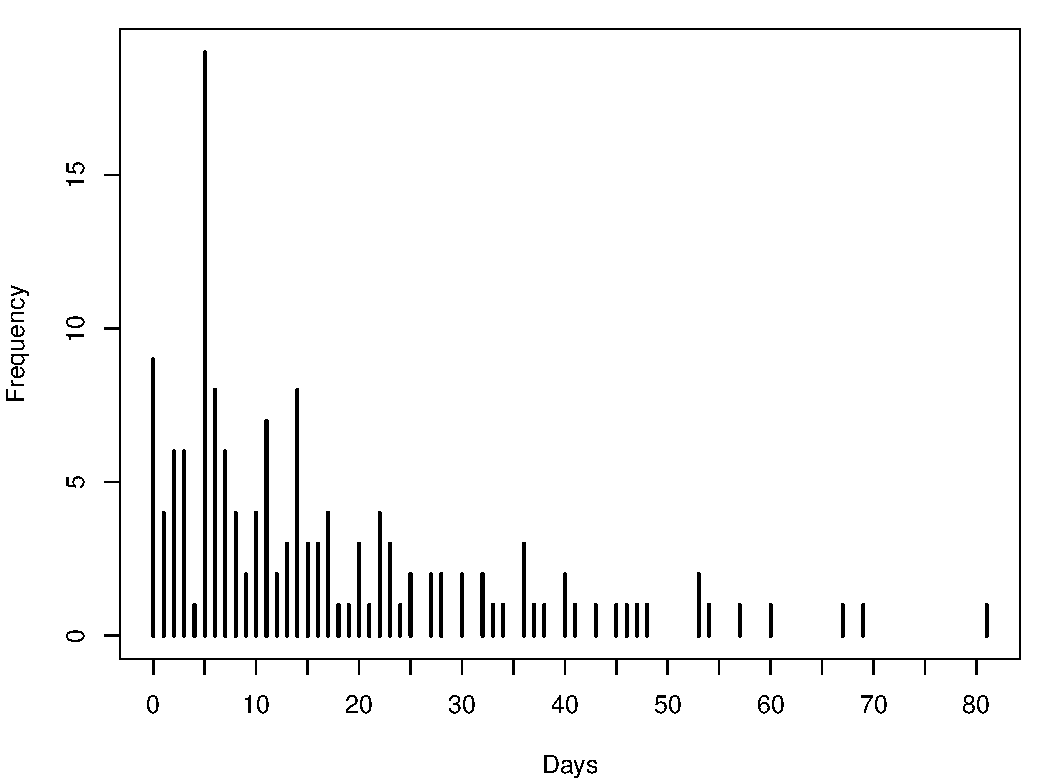
\includegraphics{article-visualization}
\caption{\label{fig:quine} Frequency distribution for number of days absent
from school.}
\end{figure}

As a first model for the \code{quine} data, we fit the basic Poisson regression
model. (Note that JSS prefers when the second line of code is indented by two
spaces.)
%
\begin{CodeChunk}
\begin{CodeInput}
R> m_pois <- glm(Days ~ (Eth + Sex + Age + Lrn)^2, data = quine,
+    family = poisson)
\end{CodeInput}
\end{CodeChunk}
%
To account for potential overdispersion we also consider a negative binomial
GLM.
%
\begin{CodeChunk}
\begin{CodeInput}
R> library("MASS")
R> m_nbin <- glm.nb(Days ~ (Eth + Sex + Age + Lrn)^2, data = quine)
\end{CodeInput}
\end{CodeChunk}
%
In a comparison with the BIC the latter model is clearly preferred.
%
\begin{CodeChunk}
\begin{CodeInput}
R> BIC(m_pois, m_nbin)
\end{CodeInput}
\begin{CodeOutput}
       df      BIC
m_pois 18 2046.851
m_nbin 19 1157.235
\end{CodeOutput}
\end{CodeChunk}
%
Hence, the full summary of that model is shown below.
%
\begin{CodeChunk}
\begin{CodeInput}
R> summary(m_nbin)
\end{CodeInput}
\begin{CodeOutput}
Call:
glm.nb(formula = Days ~ (Eth + Sex + Age + Lrn)^2, data = quine, 
    init.theta = 1.60364105, link = log)

Deviance Residuals: 
    Min       1Q   Median       3Q      Max  
-3.0857  -0.8306  -0.2620   0.4282   2.0898  

Coefficients: (1 not defined because of singularities)
            Estimate Std. Error z value Pr(>|z|)    
(Intercept)  3.00155    0.33709   8.904  < 2e-16 ***
EthN        -0.24591    0.39135  -0.628  0.52977    
SexM        -0.77181    0.38021  -2.030  0.04236 *  
AgeF1       -0.02546    0.41615  -0.061  0.95121    
AgeF2       -0.54884    0.54393  -1.009  0.31296    
AgeF3       -0.25735    0.40558  -0.635  0.52574    
LrnSL        0.38919    0.48421   0.804  0.42153    
EthN:SexM    0.36240    0.29430   1.231  0.21818    
EthN:AgeF1  -0.70000    0.43646  -1.604  0.10876    
EthN:AgeF2  -1.23283    0.42962  -2.870  0.00411 ** 
EthN:AgeF3   0.04721    0.44883   0.105  0.91622    
EthN:LrnSL   0.06847    0.34040   0.201  0.84059    
SexM:AgeF1   0.02257    0.47360   0.048  0.96198    
SexM:AgeF2   1.55330    0.51325   3.026  0.00247 ** 
SexM:AgeF3   1.25227    0.45539   2.750  0.00596 ** 
SexM:LrnSL   0.07187    0.40805   0.176  0.86019    
AgeF1:LrnSL -0.43101    0.47948  -0.899  0.36870    
AgeF2:LrnSL  0.52074    0.48567   1.072  0.28363    
AgeF3:LrnSL       NA         NA      NA       NA    
---
Signif. codes:  0 '***' 0.001 '**' 0.01 '*' 0.05 '.' 0.1 ' ' 1

(Dispersion parameter for Negative Binomial(1.6036) family taken to be 1)

    Null deviance: 235.23  on 145  degrees of freedom
Residual deviance: 167.53  on 128  degrees of freedom
AIC: 1100.5

Number of Fisher Scoring iterations: 1


              Theta:  1.604 
          Std. Err.:  0.214 

 2 x log-likelihood:  -1062.546 
\end{CodeOutput}
\end{CodeChunk}



%% -- Summary/conclusions/discussion -------------------------------------------

\section{Summary and discussion} \label{sec:summary}

\begin{leftbar}
As usual \dots
\end{leftbar}


%% -- Optional special unnumbered sections -------------------------------------

\section*{Computational details}

\begin{leftbar}
If necessary or useful, information about certain computational details
such as version numbers, operating systems, or compilers could be included
in an unnumbered section. Also, auxiliary packages (say, for visualizations,
maps, tables, \dots) that are not cited in the main text can be credited here.
\end{leftbar}

The results in this paper were obtained using
\proglang{R}~3.4.1 with the
\pkg{MASS}~7.3.47 package. \proglang{R} itself
and all packages used are available from the Comprehensive
\proglang{R} Archive Network (CRAN) at
\url{https://CRAN.R-project.org/}.


\section*{Acknowledgments}

\begin{leftbar}
All acknowledgments (note the AE spelling) should be collected in this
unnumbered section before the references. It may contain the usual information
about funding and feedback from colleagues/reviewers/etc. Furthermore,
information such as relative contributions of the authors may be added here
(if any).
\end{leftbar}


%% -- Bibliography -------------------------------------------------------------
%% - References need to be provided in a .bib BibTeX database.
%% - All references should be made with \cite, \citet, \citep, \citealp etc.
%%   (and never hard-coded). See the FAQ for details.
%% - JSS-specific markup (\proglang, \pkg, \code) should be used in the .bib.
%% - Titles in the .bib should be in title case.
%% - DOIs should be included where available.

\bibliography{refs}


%% -- Appendix (if any) --------------------------------------------------------
%% - After the bibliography with page break.
%% - With proper section titles and _not_ just "Appendix".

\newpage

\begin{appendix}

\section{More technical details} \label{app:technical}

\begin{leftbar}
Appendices can be included after the bibliography (with a page break). Each
section within the appendix should have a proper section title (rather than
just \emph{Appendix}).

For more technical style details, please check out JSS's style FAQ at
\url{https://www.jstatsoft.org/pages/view/style#frequently-asked-questions}
which includes the following topics:
\begin{itemize}
  \item Title vs.\ sentence case.
  \item Graphics formatting.
  \item Naming conventions.
  \item Turning JSS manuscripts into \proglang{R} package vignettes.
  \item Trouble shooting.
  \item Many other potentially helpful details\dots
\end{itemize}
\end{leftbar}


\section[Using BibTeX]{Using \textsc{Bib}{\TeX}} \label{app:bibtex}

\begin{leftbar}
References need to be provided in a \textsc{Bib}{\TeX} file (\code{.bib}). All
references should be made with \verb|\cite|, \verb|\citet|, \verb|\citep|,
\verb|\citealp| etc.\ (and never hard-coded). This commands yield different
formats of author-year citations and allow to include additional details (e.g.,
pages, chapters, \dots) in brackets. In case you are not familiar with these
commands see the JSS style FAQ for details.

Cleaning up \textsc{Bib}{\TeX} files is a somewhat tedious task -- especially
when acquiring the entries automatically from mixed online sources. However,
it is important that informations are complete and presented in a consistent
style to avoid confusions. JSS requires the following format.
\begin{itemize}
  \item JSS-specific markup (\verb|\proglang|, \verb|\pkg|, \verb|\code|) should
    be used in the references.
  \item Titles should be in title case.
  \item Journal titles should not be abbreviated and in title case.
  \item DOIs should be included where available.
  \item Software should be properly cited as well. For \proglang{R} packages
    \code{citation("pkgname")} typically provides a good starting point.
\end{itemize}
\end{leftbar}

\end{appendix}

%% -----------------------------------------------------------------------------


\end{document}
